\documentclass[12pt]{report}
\usepackage[utf8x]{inputenc}
\usepackage[russian]{babel}
\usepackage{amsmath}
\usepackage{graphicx}

\graphicspath{{graphic/chapter2/}}

\renewcommand{\labelenumii}{\arabic{enumi}.\arabic{enumii}}

\textwidth=15cm
\textheight=22cm
\oddsidemargin= 0.5cm
\topmargin = -0.5cm


\begin{document}

\newpage

    \section{Анализ предметной области.}
    \subsection{Описание структуры сети.}

    В настоящее время можно выделить несколько типов сетей:
    \begin{itemize}
        \item персональные сети;
        \item локальные сети;
        \item муниципальные сети;
        \item глобальные сети;
    \end{itemize}

    \subsubsection{Персональные сети. }

    Персональные сети (PAN) позволяют общаться устройствам вблизи человека. Типичный пример - беспроводная сеть, которая соединяет компьютер с его периферийными устройствами. Почти у каждого компьютера есть присоединенный монитор, клавиатура, мышь и принтер. При отсутствии беспроводной сети они должны быть присоединены кабелями. Примером беспроводной сети может служить беспроводная сеть малой дальности Bluetooth.

    В самой простой форме сети Bluetooth используют парадигму ведущий-ведомые(Master-Slave). Системный модуль (PC) обычно является ведущим устройством и общается с мышью, клавиатурой и.т.д. как с ведомыми устройствами. Ведущее устройство сообщает ведомым какие адреса использовать, когда они могут осуществлять широковещательную передачу, сколько времени они могут передавать, какие частоты использовать и.т.д.

    \subsubsection{Локальные сети.}
    Локальными сетями называют частные сети, размещающиеся, как правило, в одном здании или на территории какой-либо организации. Их часто используют для для объединения компьютеров и рабочих станций в офисах компании или предприятия для предоставления совместного доступа к ресурсам и обмена информацией. Беспроводные ЛВС сейчас очень популярны, особенно в домах, более старых офисных зданиях, кафетериях и других местах, где слишком сложно провести кабели.

    Стандарт для беспроводных ЛВС, названный IEEE 802.11, более известный как WiFi, стал очень широко распространен. Он работает на скоростях от 11 до 100 мегабит в секунду.

    В проводных ЛВС используют различные технологии передачи. Большинство из них использует медные провода, а некоторые - оптоволокно. ЛВС ограничены в размере, это означает, что максимальное время передачи ограничено и известно заранее.

    Топология многих проводных сетей создана из магистральных линий. Стандарт IEEE 802.3, обычно называемый Ethernet, является наиболее распространенным типом проводной ЛВС.

    И проводные и беспроводные широковещательные сети в зависсимости от способа назначения канала подразделяются на статические и динамические. При статическом назначении используется циклический алгоритм, и все время делится между всеми машинами на равные интервалы, так что машина может передавать данные только в течении выделенного ей интервала времени. При этом емкость канала расходуется не эффективно, так как временной интервал предоставляется машинам вне зависимости от того, есть ли у них данные для передачи.

    Методы динамического предоставления доступа к каналу так же могут быть централизованными и децентрализованными. При централизованном методе предоставления доступа к каналу должно существовать одно устройство, определяющее машину, получающую право на передачу. Оно должно получать множество пакетов и принимать решение о приоритетах на основании внутреннего алгоритма. При децентрализованном методе каждая машина сама принимает решение о необходимости передачи данных.


    \subsubsection{Муниципальные сети. }
    Муниципальные сети (metropolital area network, MAN) объединяет компьютеры в пределах города. Самым распространенным примером муниципальной сети является система кабельного телевидения. В стандарте IEEE 802.16 описана MAN известная всем как WiMax

    \subsubsection{Глобальные сети. }

    Глобальные сети (wide area networks, WAN) охватывает значительную географическую область, часто целую страну или даже континент. В состав такой сети входят машины, называемые хостами. Они объединяются в подсети, задача которых - передача трафика от хоста к хосту.

    В большинстве глобальных сетей подсеть состоит из двух раздельных компонентов: линий связи и переключающих компонентов. Линии связи предназначены для передачи данных от машине к машине, в то время как переключающие компоненты необходимы для соединения линий связи. В качестве линий связи используются медный провод, оптоволокно или радиосвязь.

    \subsection{Иерархия протоколов. }

    Для упрощения структуры большинство сетей организуется в наборы уровне, каждый последующий является надстройкой над предыдущим. Количество уровней, их название, содержание и назначение разные и зависят от сети. Целью каждого уровня явлется предоставление неких сервисов для вышестоящих уровней. При этом детали реализации остаются скрытыми.

    На рисунке \ref{Pic1} показана пятиуровневая сеть. Взаимодействие между объектами одного уровня не происходит на прямую. Взаимодействующие уровни передают данные нижестоящему протоколу. Так продолжается до самого нижнего уровня. Ниже первого уровня - физическая среда, по которой и происходит обмен информацией.

    \begin{figure}\center
        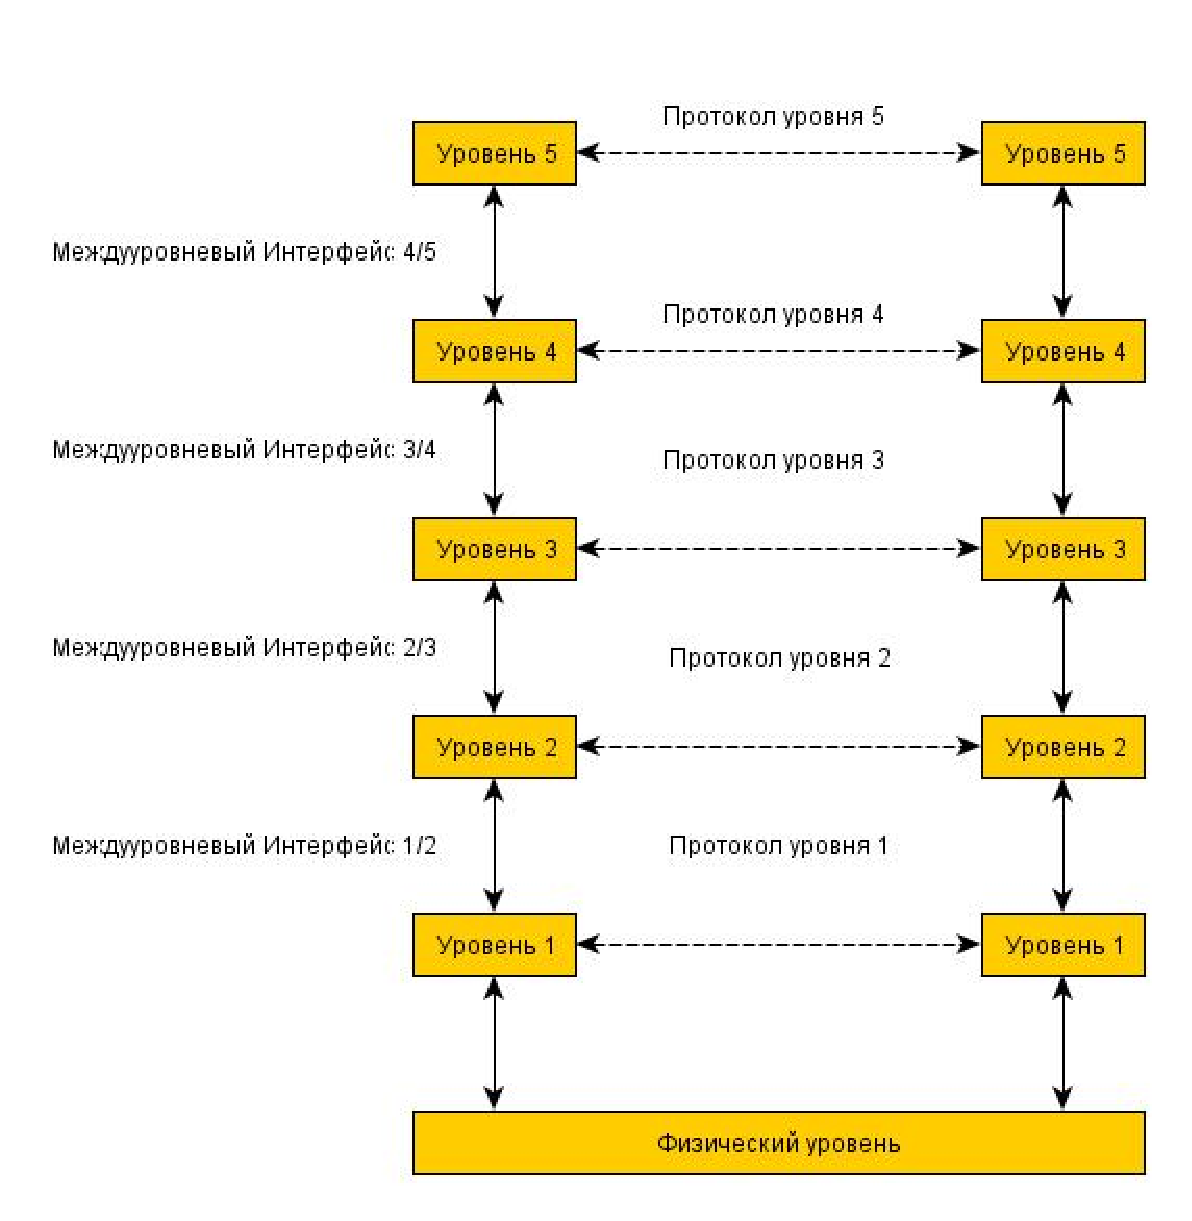
\includegraphics[width = 120mm]{Ch2Pic1}
        \caption{Пятиуровневый стек протоколов.} \label{Pic1}
    \end{figure}

    Набор уровней и протоколов называется архитектурой сети. Спецификация архитектуры должна содержать достаточно информации для написания программного обеспечения или создания аппаратуры для каждого уровня, чтобы они корректно выполняли требования протокола. Ни детали реализации, ни спецификация интерфейсов не являются частями архитектуры. При этом не требуется, чтобы интерфейсы на на всех машинах сети были одинаковыми, необходима только корректная обработка данных этими интерфейсами. Список протоколов, используемых системой, по одному протоколу на уровень, называется стеком протоколов.

    \subsection{Эталонные модели взаимодействия.}

    \subsubsection{Эталонная модель OSI.}

    Эталонная модель OSI(open systems interconnection), за исключение физической среды показана на рисунке \ref{Pic2}. Эта модель имеет семь уровней. Появление именно такой структуры было обусловлено следующими соображениями.
    \begin{itemize}
        \item Уровень должен создаваться по мере необходимости отдельного уровня абстракции.
        \item Каждый уровень должен выполнять строго определенную функцию.
        \item Выбор функций для каждого уровня должен осуществляться с учетом создания стандартизированных международных протоколов.
        \item Границы между уровнями должны выбираться так, чтобы поток данных между интерфейсами был минимальным.
        \item Количество уровней должно быть достаточно большим, чтобы различные функции не объединялись в одном уровне без необходимости, но не слишком высоким, чтобы архитектура не становилась громоздкой.
    \end{itemize}

    \begin{figure}[H]\center
        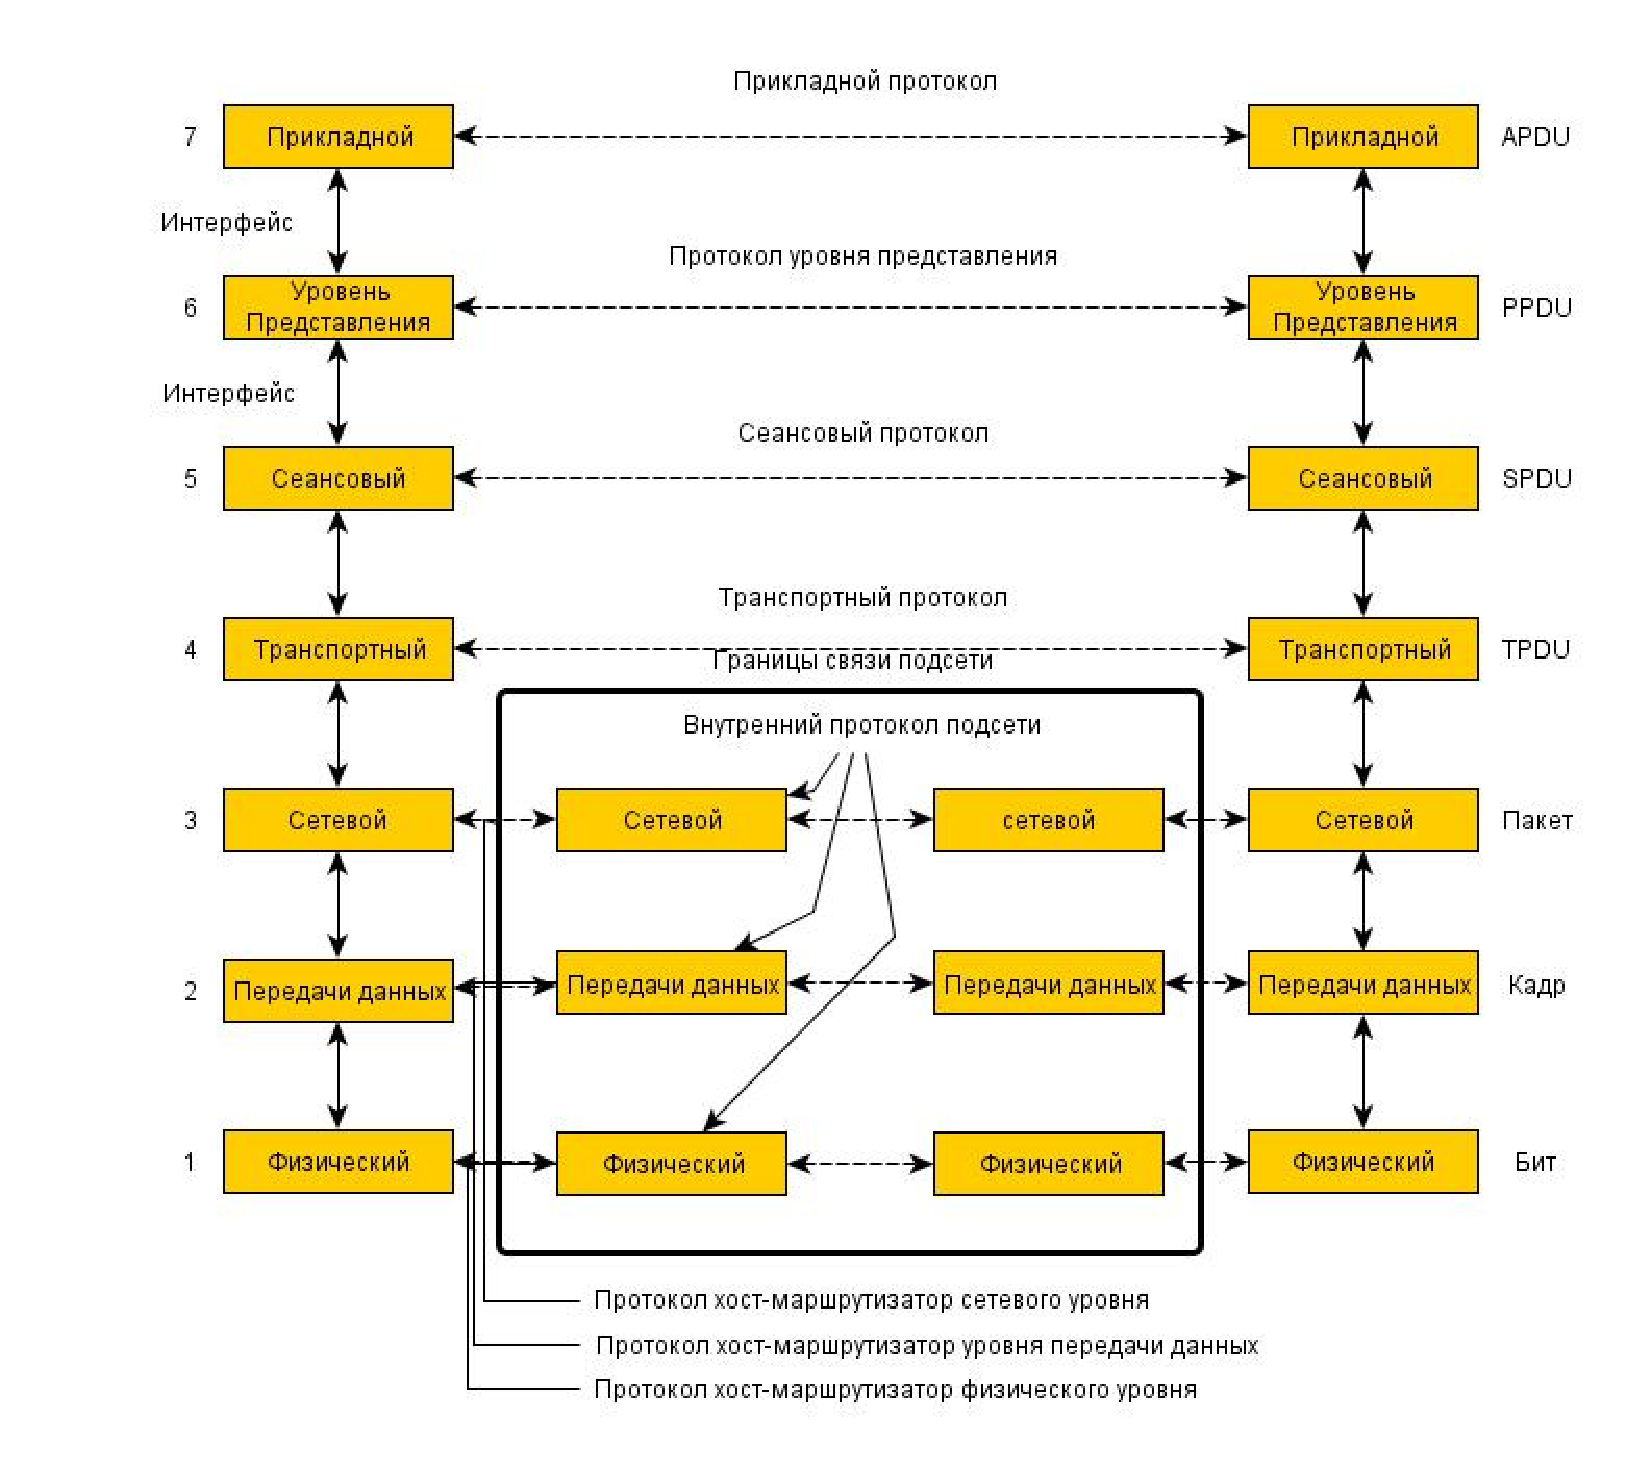
\includegraphics[width = 140mm]{Ch2Pic2}
        \caption{Эталонная модель взаимодействия открытых систем.} \label{Pic2}
    \end{figure}

    Далее представлено краткое описание каждого уровня рассматриваемой модели.

    \begin{itemize}
        \item Физический уровень. Физический уровень занимается реальной передачей необработанных битов по каналу связи. На данном уровне определяются такие параметры как соответствие напряжения и передаваемого значения, длительность единичного сигнала, направление передачи(дуплекс, полу-дуплекс), начало и окончание передачи сигнала, характеристики канала связи.
        \item Уровень передачи данных. Основная задача -- быть способным передавать "сырые" данные физического уровня по надежной линии связи, свободной от необнаруженных ошибок и маскировать реальные ошибки так, что сетевой уровень их не видит. Эта задача выполняется при помощи разбиения входных данных на кадры,обычный размер которых колеблется от нескольких сот до нескольких тысяч байт.
        \item Сетевой уровень. Сетевой уровень занимается управлением операциями подсети. Важнейшим моментом здесь является определение маршрутов пересылки от источника к пункту назначения. Маршруты могут быть жестко заданы в виде таблиц и редко меняться либо, что бывает чаще, динамически меняться чтобы избегать отказавших компонентов.
        \item Транспортный уровень. Основная функция транспортного уровня - принять данные от сеансового уровня, разбить их при необходимости на небольшие части, передать их сетевому уровню., и гарантировать, что эти части прибудут в правильном виде прибудут по назначению.
        \item Сеансовый уровень. Сеансовый уровень позволяет пользователям различных компьютеров устанавливать сеансы связи друг с другом. При этм предоставляются различные типы сервисов.
        \item Уровень представления. Данный уровень занимается синтаксисом и семантикой передаваемой информации. Чтобы было возможно взаимодействие компьютеров с различным внутренним представлением данных, необходимо преобразовывать форматы данных друг в друга, передавая их по сети в неком стандартизованном виде.
        \item Прикладной уровень. Прикладной уровень содержит набор популярных протоколов, необходимых пользователю.
    \end{itemize}

\subsubsection{Эталонная модель TCP/IP. }

    Главной целью возникновения новой архитектуры стало требование объединения различных сетей, для чего от новой архитектуры требовалась гибкость и возможность взаимодействия с существовавшими на тот момент протоколами. Все эти требоания привели к выбору сети с коммутацией пакетов, основанной на уровне без установления соединения, который работает в различных сетях. Рассмотрим уровни, используемые в этой модели (Рисунок \ref{Pic3}).

    \begin{itemize}
        \item Канальный уровень. Данный уровень описывает то, как и что каналы, такие как последовательные линии и классический Ethernet, должны сделать чтобы удовлетворить потребности межсетевого уровня без установления соединения.
        \item Межсетевой уровень. Задача этого уровня заключается в обеспечении возможности каждого хоста посылать пакеты в любую сеть и независимо двигаться к пункту назначения.
        \item Транспортный уровень. Этот уровень создан для того, чтобы объекты одного ранга на приемных и передающих хостах могли поддерживать связь.
        \item Прикладной уровень. Содержит в себе функции сеансового уровня и уровня представления модели OSI, а также пользовательские протоколы высокого уровня.
    \end{itemize}

    \begin{figure}\center
        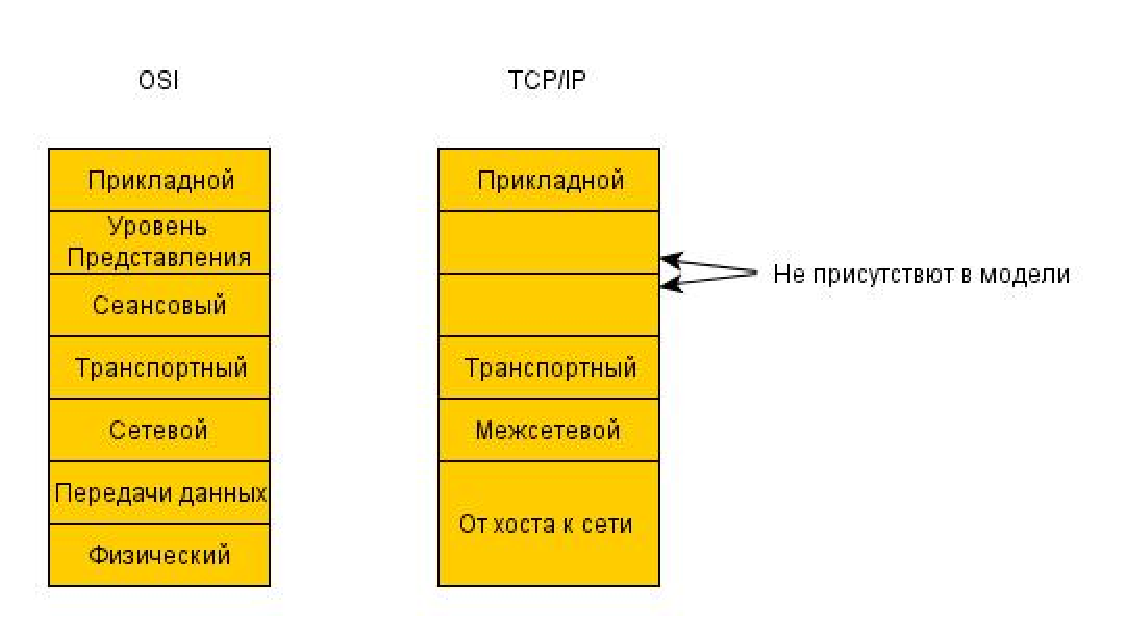
\includegraphics[width = 120mm]{Ch2Pic3}
        \caption{Эталонная модель TCP/IP.} \label{Pic3}
    \end{figure}

    При разработке модели локальной сети для проектируемой системы будет использована гибридная модель, сочетающая в себе достоинства обоих описанных подходов. Уровни используемой модели показаны на рисунке \ref{Pic4}.

    \begin{figure}\center
        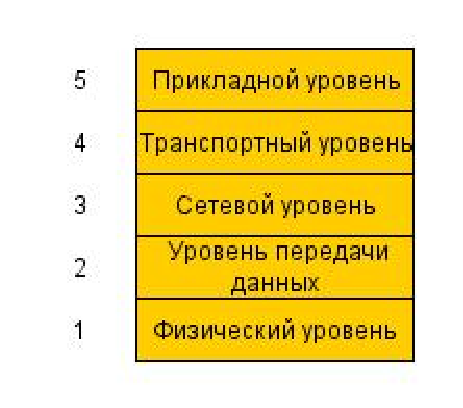
\includegraphics[width = 50mm]{Ch2Pic4}
        \caption{Модель сетевого взаимодействия, используемая при разработке.} \label{Pic4}
    \end{figure}

    \subsection{Сетевые устройства. }

    Для обеспечения передачи информации между рабочими станциями, т.е. объединения их в сеть применяются различные устройства. Для удобства их перечисление и описание принципов работы приведено в соответствии используемой моделью сетевого взаимодействия. Для описания процесса взаимодействия между рабочими станциями, необходимо так же описать принцип работы протокола соответствующего уровня.

    \subsubsection{Устройства, взаимодействующие на физическом уровне}

    Физический уровень работы сети связан непосредственно с процессом передачи сигнала. Каждое устройство передачи данных в сети имеет элемент, который преобразует данные в сигнал и передает его. так же это устройство отвечает за прием входящих сигналов.

    Для передачи сигналов от одного передатчика к другому необходим канал связи. При построении локальных сетей используется несколько способов, таких как: беспроводная передача данных и передача данных с использованием соединительных проводов.

    Соединительные провода могут быть разных типов, и обеспечивать различные характеристики передачи сигналов. Например: витая пара, оптоволокно, коаксиальный кабель.

    \subsubsection{Канальный уровень взаимодействия. }

    Канальный уровень является логическим уровнем, надстройкой над физическим уровнем. Протокол, работающий на этом уровне решает две основные задачи: контроль среды передачи данных и формирования кадров. Стандарт Ethernet выделяет два подуровня на канальном уровне: MAC и LLC. LLC-подуровень отвечает за формирование кадров и контроль адресов входящих и исходящих передач. MAC(Media Access Control) отвечает за передачу кадров, полученных от LLC-подуровня, через канал связи.

    В случае централизованного контроля передачи данных, проблема разделения среды не возникает. Однако следует рассмотреть вариант децентрализованной передачи, при котором каждая рабочая станция сама принимает решение о необходимости пересылки данных.

    Для примера рассмотрим так называемый классический Ethernet. В качестве среды передачи данных при использовании этого протокола используется так называемая шина -- проводник к которому подключены несколько рабочих станций. Для передачи данных, устройство, контролируемое протоколом MAC-подуровнем "прослушивает" канал связи. В тот момент, когда канал связи является свободным, сетевое устройство начинает передачу данных. При такой реализации возможна проблема одновременного начала передачи несколькими рабочими станциями.

    Для решения такой проблемы используется метод контроля несущей и обнаружения столкновений(CSMA/CD). В случае если в момент исходящей передачи обнаружена входящая, передача прекращается, а в КС посылается jam-последовательность для того, чтобы остальные рабочие станции обнаружили коллизию. Для того, чтобы осуществить передачу и избежать повторной коллизии используется экспоненциальный двоичный алгоритм выдержки, который определяет временную интервал, по истечении которого будет предпринята повторная попытка передачи. Подробнее этот алгоритм будет описан при построении моделей устройств.

    В настоящее время в основном используется коммутируемый Ethernet. Его основное отличие от классического состоит в том, что устройства, объединенные в сеть, подключаются не к общему проводнику, а к устройству, называемому коммутатором(switch). И в случае, если используется дуплексный режим передачи, то коллизий не возникает. Однако, в случае использования полу-дуплексного режима работы, коллизии обрабатываются в соответствии с описанным методом.

    Коммутатор - это устройство, работающее на канальном уровне используемой модели взаимодействия, объединяющее устройства в сеть и отвечающее за пересылку пакетов от отправителя к получателю. Для этого используется таблица коммутации, которая представляет собой соотношение "адрес-порт" и позволяет передавать пакеты не по всей сети а только получателю. при рассмотрении процесса работы коммутатора можно выделить два режима работы.

    \begin{itemize}
        \item режим обучения, во время которого составляется таблица коммутации. Каждому порту ставится в соответствие адрес отправителя, подключенного к этому порту. При этом, если неизвестен порт, к которому подключен получатель, ведется широковещательная рассылка.
        \item Основной режим работы. В этом режиме все пакеты, кроме обозначенных как широковещательные, передаются только получателю.
    \end{itemize}

    \subsubsection{Сетевой уровень взаимодействия. }

    Основной задачей, решаемой протоколами сетевого уровня являются задачи маршрутизации пакетов в сети.
    %Возможно стоить добавить общее описание алгоритма маршрутизаци. Хотя он все равно будет в Гл.3.
    Маршрутизатор.

    \subsubsection{Транспортный уровень взаимодействия. }

    Конечная цель транспортного уровня заключается в предоставлении эффективных надежных и экономичных услуг(сервисов) передачи данных своим пользователям, которыми обычно являются процессы прикладного уровня. Сервисы транспортного уровня, как и сервисы сетевого уровня, делятся на сервисы с установлением соединения и без установления соединения. Транспортный сервис с установлением соединения во многом похож на аналогичный сервис сетевой сервис. Основным отличием сервисов транспортного уровня является надежность передачи данных.

    \section{Построение моделей. }

    \subsection{Общая модель сети. Среда.}

        %Общие слова про модель среды, про создание и поддержку существования моделей отдельные объектов.

    Локальная сеть представляет собой соединенные рабочие станции, взаимодействие между которыми осуществляется посредством сетевых протоколов. Общая модель сети является результатом взаимодействия моделей объектов, входящих в ее состав. В связи со сложностью моделирования некоторых процессов, необходимо использовать упрощенные модели. Такими процессами являются например ошибки в каналах связи или процесс генерации пользователем сетевого трафика. Напротив, протоколы взаимодействия представляют собой алгоритмы поведения при обработке данных и, таким образом, представляется возможным создать модели, отражающие это поведение достаточно точно.

    \subsection{Модели устройств.}

    Любое устройство, входящее в состав локальной сети взаимодействует с остальными используя соответствующие протоколы. Это позволяет выделить два основных процесса при обмене данными: обработка приема и передачи данных, т.е. непосредственно работа сетевых протоколов, и обработка полученной информации приложением или алгоритмом, в зависимости от устройства, которым данные получены (рисунок \ref{Pic5}).

    \begin{figure}\center
        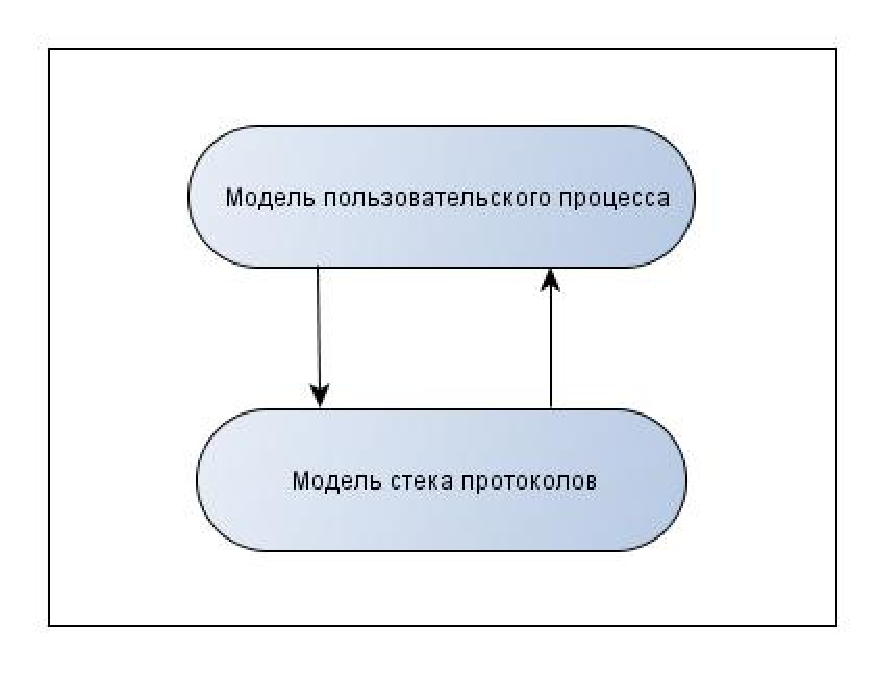
\includegraphics[width = 60mm]{Ch2Pic5}
        \caption{Общий вид модели устройства.} \label{Pic5}
    \end{figure}

    \subsubsection{Модель канала связи. }

    В реальной системе, связанной с передачей данных, всегда существует некоторая вероятность появления ошибки при прохождении сигнала через канал связи. Существует несколько различных моделей каналов связи, обладающих различными характеристиками и по-разному моделирующих ошибку. В рамках разрабатываемой системы используем абстракцию для модели канала связи, обладающую следующими характеристиками:

    \begin{itemize}
        \item доступ к КС может быть получен любым из подключенных устройств в любой момент времени;
        \item передача сигнала всегда происходит с некоторой задержкой;
    \end{itemize}

    Подобная модель позволит строить модель сети с использованием идеального канала связи без помех. Возможность же моделировать ошибку при прохождении сигнала реализуется моделью, которая может входить или не входить в состав представленной.

    \subsubsection{Модель стека сетевых протоколов. }

    Модель протокола взаимодействия представляет собой алгоритм обработки данных полученных с нижнего или верхнего уровней. Однако, для правильной организации обмена информацией посредством сети, необходимо объединить используемые протоколы в сеть. Так как разрабатываемая система не подразумевает использование каких-то конкретных протоколов и должна предоставлять возможности для моделирования различных вариантов, то необходимо построить модель абстрактного протокола, при этом реализовав возможность изменения способа обработки данных. Любой протокол предоставляет возможность вышестоящему протоколу отправить данные и принять данные от нижестоящего протокола. Наиболее общая модель протокола представлена на рисунке \ref{Pic6}.
    \begin{figure}\center
        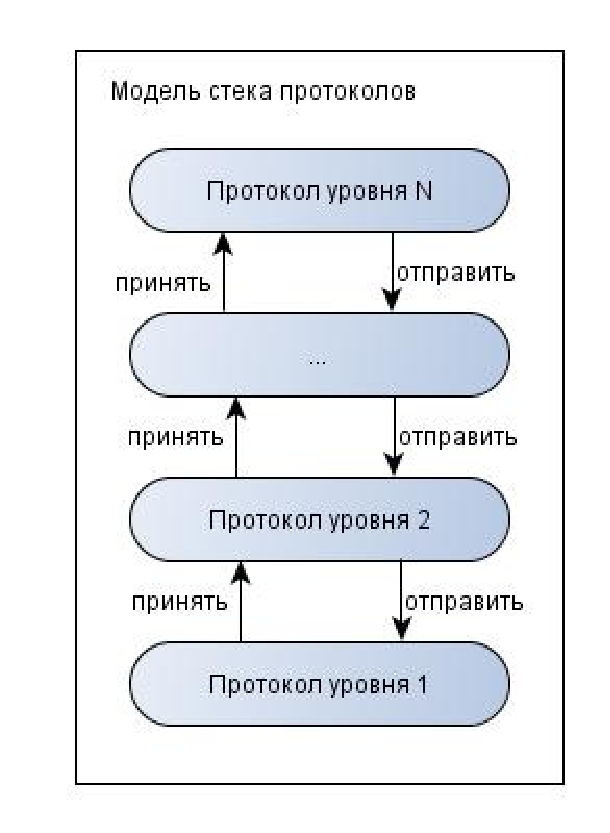
\includegraphics[width = 70mm]{Ch2Pic6}
        \caption{Модель взаимодействия протоколов.} \label{Pic6}
    \end{figure}
    В качестве отдельного типа протоколов можно выделить протоколы, управляющие средой передачи данных. Особенностью таких протоколов является методы контроля за процессом передачи данных, решение возникающих при передаче конфликтов и управления устройством передачи данных. Учитывая эти требования, модель протокола управления средой передачи данных может быть изображена следующим образом(рисунок \ref{Pic7})
    \begin{figure}\center
        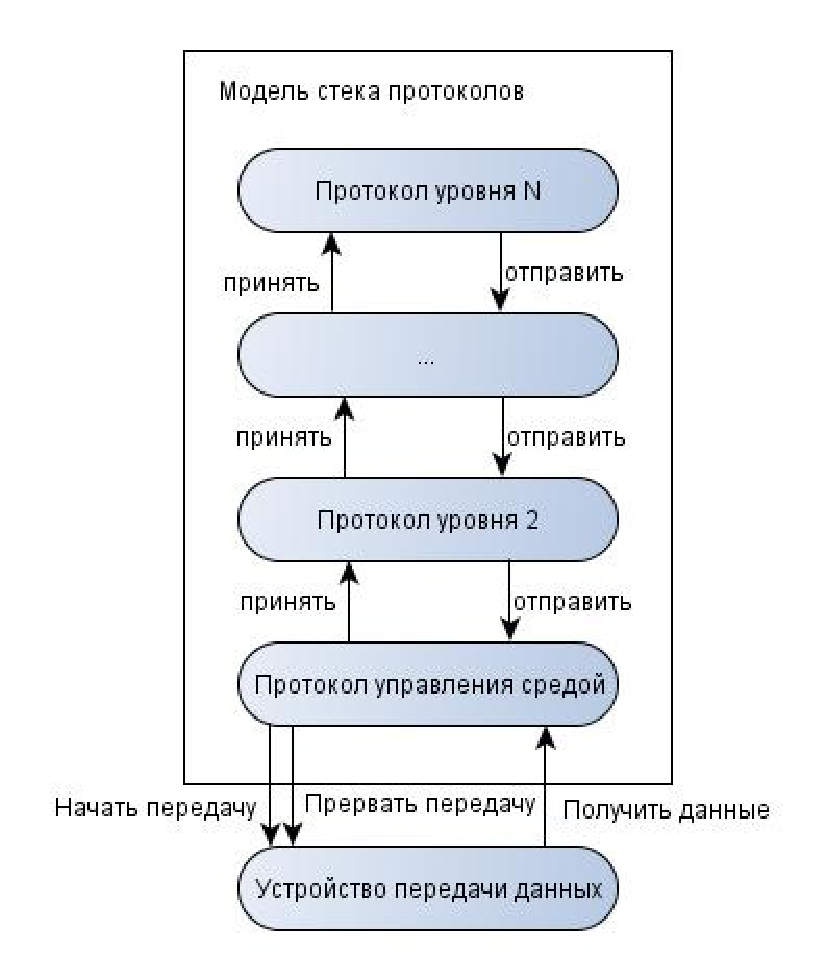
\includegraphics[width = 70mm]{Ch2Pic7}
        \caption{Модель взаимодействия стека протоколов со средой.} \label{Pic7}
    \end{figure}
    В некоторых случаях, следует так же выделить в отдельный тип протоколы, используемые на транспортном уровне. В рамках используемой модели взаимодействия, транспортная подсистема представляет собой несколько алгоритмов обработки данных, реализация которых скрыта от пользователя. Для осуществления взаимодействия приложению предоставляется интерфейс, методы которого перечислены в таблице.

    %Сделать нумерацию таблиц.

    \begin{tabular}{|c|c|}
        \hline
        LISTEN & ожидание соединения \\ \hline
        CONNECT & активное установление соединение \\ \hline
        SEND & отправка данных \\ \hline
        RECEIVE & ожидание получения данных \\ \hline
        DISCONNECT & Прервать соединение \\ \hline

    \end{tabular}


    Кроме описанных протоколов, в стеке иногда применяются протоколы для установления соответствия между адресами, используемыми на разных уровнях модели. Такие протокол не связны с приложениями, но связаны с протоколами уровней ниже транспортного. Для адресации на нижних уровнях сети используется MAC-адрес рабочей станции - уникальный идентификатор присваиваемый каждой единице оборудования компьютерных сетей. Но для осуществления взаимодействия между приложениями используются адреса более высоких уровней. Для того, чтобы решить подобную проблему, используют протоколы, которые устанавливают и хранят соответствие между адресами для каждого собеседника. Данный вид взаимодействия изображен на рисунке
    \ref{Pic8}.
    \begin{figure}\center
        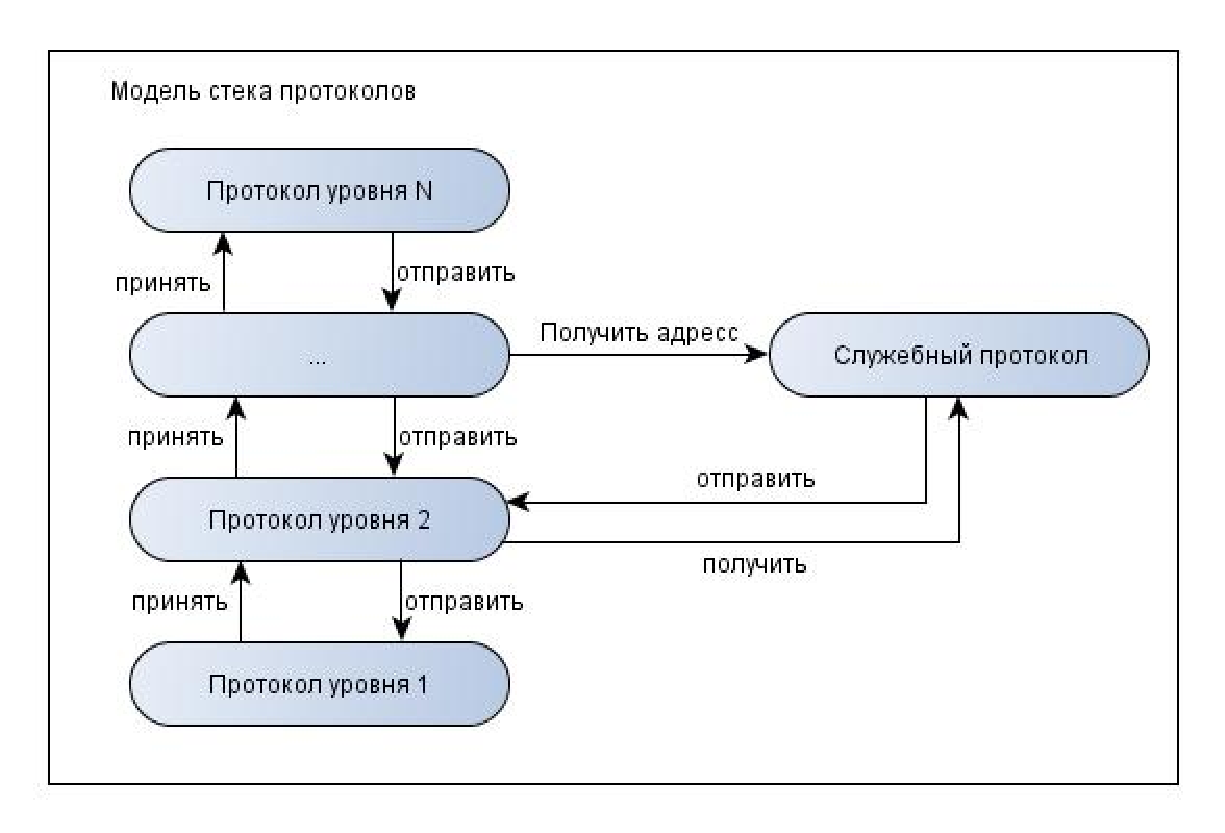
\includegraphics[width = 70mm]{Ch2Pic8}
        \caption{Модель взаимодействия служебных протоколов.} \label{Pic8}
    \end{figure}

    Модель любого из описанных протоколов представляет собой конечный автомат. Количество состояний и функции перехода зависят непосредственно от реализации протокола. Так для протоколов сетевого и транспортного уровня с установлением соединения, количество состояний определяется используемыми алгоритмами установления соединений, обмена данными и разрыва соединений.

    Принцип взаимодействия протоколов показан на рисунке \ref{Pic9}.

    \begin{figure}\center
        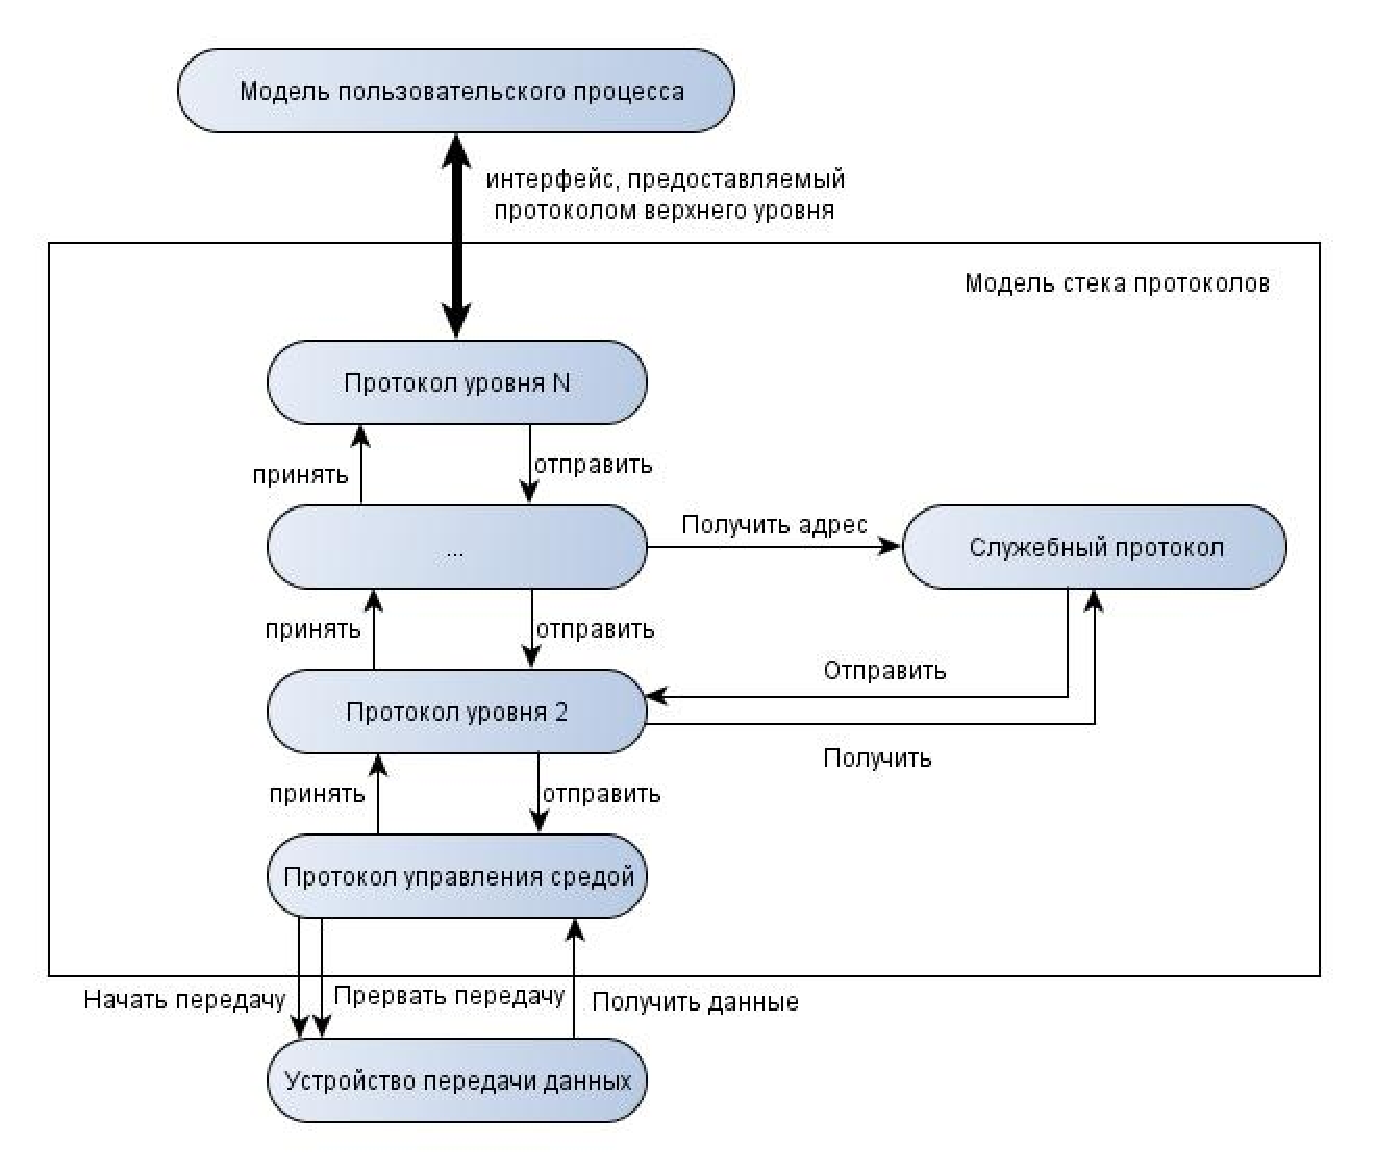
\includegraphics[width = 120mm]{Ch2Pic9}
        \caption{Пятиуровневый стек протоколов.} \label{Pic9}
    \end{figure}

    \subsection{Моделирование пользовательских процессов. }

    Характер сетевого взаимодействия и, следовательно, сетевой трафик, определяется задачами, решаемыми пользователем с использованием рабочей станции и сетевых ресурсов. Оценки характеристик сети передачи данных необходимо иметь возможность моделировать ее поведение в различных ситуациях. Для моделирования нормального режима работы необходимо построить модель генератора трафика, которая будет имитировать нагрузку, близкую по интенсивности и характеру к той, которая генерируется в локальной сети. Моделирование атак различного рода подразумевает подключение к сети злоумышленника, с рабочей станции которого и производится воздействие на компоненты сети. Так же атаки могут быть реализованы с помощью сети интернет, при наличии соответствующего подключения.

    В общем случае пользовательский процесс представляет собой объект, использующий сетевое подключение для обмена информацией с другими процессами. Так как процессы в исследуемой сети рассматриваются с точки зрения оценки нагрузки, то характер передаваемых данных не имеет значения. Поэтому для имитации пользовательской активности используем модели генераторов сетевого трафика, а передаваемые данные будут случайными последовательностями бит.

    Отдельно рассматриваются действия злоумышленника. Для моделирования различного рода атак, пользовательские процессы злоумышленника должны иметь возможность обмениваться "осмысленными" данными с рабочими станциями, и на основе этих данных реализовать имитацию атаки.

    Используемая модель пользовательского процесса представлена на рисунке \ref{Pic10}

    \begin{figure}\center
        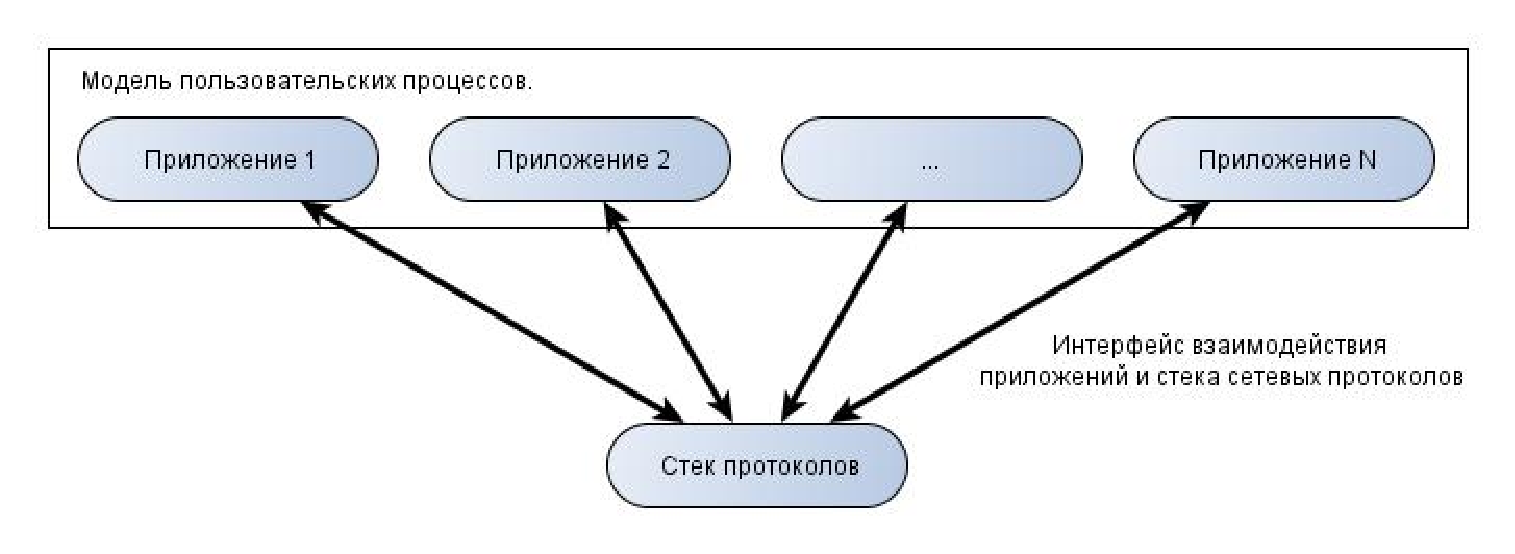
\includegraphics[width = 120mm]{Ch2Pic10}
        \caption{Пятиуровневый стек протоколов.} \label{Pic10}
    \end{figure}

    \subsubsection{Модель поведения пользователя. }

    Поведение пользователя представлено в модели посредством моделей генерации сетевого трафика. Методы моделирования сетевого трафика можно концептуально разделить на аналитические и имитационные. Аналитическое моделирование подразумевает формальное описание моделируемых объектов и процессов в виде совокупности математических уравнений и выражений. Данные модели удобны для проведения теоретических исследований и формальных манипуляций, однако, в большинстве случаев построение адекватной аналитической модели для многих видов сетевого трафика является практически невыполнимой задачей.

    В том случае, если моделирование ставит перед собой задачу вычисления(оценку) рабочих характеристик параметров моделируемой системы, наиболее предпочтительным является использование имитационных моделей.

    На сегодняшний день можно выделить четыре класса моделей, применяемых для моделирования сетевого трафика:
    \begin{itemize}
        \item использующие классические модели потоков, применяемые в теории массового обслуживания;
        \item основанные на так называемых модулированных случайных процессах;
        \item учитывающие статистическое самоподобие некоторых видов трафика;
        \item строящие имитационные последовательности по образцу трафика.
    \end{itemize}

    Наиболее перспективными на сегодняшний день считаются модели на основе обобщенных модулированных случайных процессов(Generally Modulated Process - GMP) и фрактальные модели на основе хаотических отображений.

    Последние исследования сетей с коммутацией пакетов говорят о статистическом самоподобии некоторых видов трафика и наличии эффекта долгосрочной зависимости.

    Самоподобный трафик обладает следующими статистическими свойствами, важными с точки зрения моделирования:
    \begin{itemize}
        \item распределения временных промежутков поступления пакетов медленно убывают и имеют т.н. "тяжелые хвосты";
        \item распределения временных промежутков поступления пакетов обладают бесконечными моментами(начиная с некоторого порядка);
        \item медленной скоростью ($n_{-1}$) убывания дисперсии вычисленной на основе образца трафика при увеличении длины образца;
    \end{itemize}

    Следует отметить, что в условиях самоподобного трафика классические методы расчета параметров компьютерной сети(пропускной способности каналов, емкости буферов и пр), основанные на пуассоновских потоках, зачастую дают неоправданно оптимистические решения и приводят к недооценки нагрузки.

    Фрактальные модели. Наиболее распространенными моделями, предназначенными для имитации фрактального трафика, являются:

    \begin{itemize}
        \item хаотические отображения;
        \item фрактальное броуновское движение;
        \item фрактальный гауссовский шум;
    \end{itemize}

    Наиболее распространенными и концептуально простыми простыми моделями, позволяющими генерировать самоподобный трафик, являются модели, построенные на так называемый хаотических отображениях(CMAPs). Эти модели используют меньшее число параметров, чем два других метода, и их выбор имеет более наглядную трактовку.

    Одномерное отображение $
        x_{n+1} = \left\{
                    \begin{aligned}
                        f_{1}(n), 0 < x_{n} <= d \\
                        f_{2}(n), d < x_{n} < 1 \\
                    \end{aligned}
                  \right. $
    , где d - параметр отображения называется хаотическим, если функции $f_{1}$ и $f_{2}$ удовлетворяют условию чувствительности к начальным условиям, т.е. расстояние между траекториями через N последовательных итераций можно записать в форме $\|f^{N}(x_{0} + \delta) - f^{N}(x_{0})\| = \delta \cdot e^{N\lambda(x_{0})}$, где $\lambda(x_{0}) > 0$ для большинства значений $x_{0}$.

    Одним из наиболее используемых отображений является последовательность "перемежаемость"

    $$
        x_{n+1} = \left\{
                    \begin{aligned}
                        \epsilon + x_{n} + cx_{m}^{n}, 0 < x_{n} < d, \\
                        \dfrac{x_{n} - d}{1 - d}, d < x_{n} < 1\\
                    \end{aligned}
                  \right.
    $$
    где $c = \dfrac{1 - \epsilon - d}{d_{m}}$.

    Варьируя параметр $\epsilon$ можно изменять продолжительность нахождения модели в первом состоянии, при помощи параметров d и m можно управлять средним значением интенсивности трафика.

    \subsubsection{Построение моделей атак. }

    Для моделирования вредоносной активности, рассмотрим два класса атак, применимых в сетях передачи данных.

    В первый класс выделены атаки типа "отказ в обслуживании", спуфинг, т.е. атаки на сетевые протоколы и оборудование. Атаки, принадлежащие к этому классу, ориентированы на протоколы. Для проведения такой атаки, злоумышленник генерирует трафик определенной интенсивности и структуры. Под структурой понимается внутренне строение используемых пакетов. Данный вид атак направлен на использование особенностей работы протоколов в целях получения доступа к передаваемым по сети данным(спуфинг) или повышение интенсивности трафика в сети, что приводит к росту очередей на устройствах обработки данных и снижению производительности сети(атаки типа "отказ в обслуживании"). Таким образом модель представляет собой алгоритм генерации трафика соответствующего назначения.

    Вторым классом атак, рассматриваемых в системе являются атаки на рабочие станции с использованием уязвимостей приложений. Условно процесс атаки на рабочую станцию можно разбить на несколько этапов:

    \begin{itemize}
        \item Сбор информации. Успех атаки напрямую зависит от возможности получить информацию о целевой сети(используемые адреса, операционные системы и доступные сервисы.)
        \item Атака. На этом этапе злоумышленник использует собранную на предыдущем этапе информацию, определяет порядок действий и создает эксплойт. Эксплойт -- это программа, которая внедряет исполняемый код в уязвимую систему.
        \item Сбор информации с использованием доступа к системе. На этом этапе злоумышленник имеет возможности для получения информации, к которой он не имел доступа до компрометации системы.
        \item Повышение привилегий. Используя уязвимости на скопрометированной системе, злоумышленник пытается получить права администратора на локальной машине.
        \item Развертывание. Злоумышленник может использовать доступ к рабочей станции для дальнейшей атаки на другие узлы сети.
        \item Сокрытие следов. На этом этапе злоумышленник скрывает следы свое присутствия в системе.
    \end{itemize}

    Для построения модели ограничимся рассмотрением двух первых этапов атаки: сбор информации и процесс атаки. Модель приложений схематично изображена на рисунке \ref{Pic12}. Каждое приложение представляет собой объект, который может быть использован для атаки атаки на систему. Объекты разделяются на два вида:

    \begin{itemize}
        \item объекты, содержащие уязвимость;
        \item объекты, содержащие информацию, которую можно использовать для эксплуатации уязвимости.
    \end{itemize}


    \begin{figure}\center
        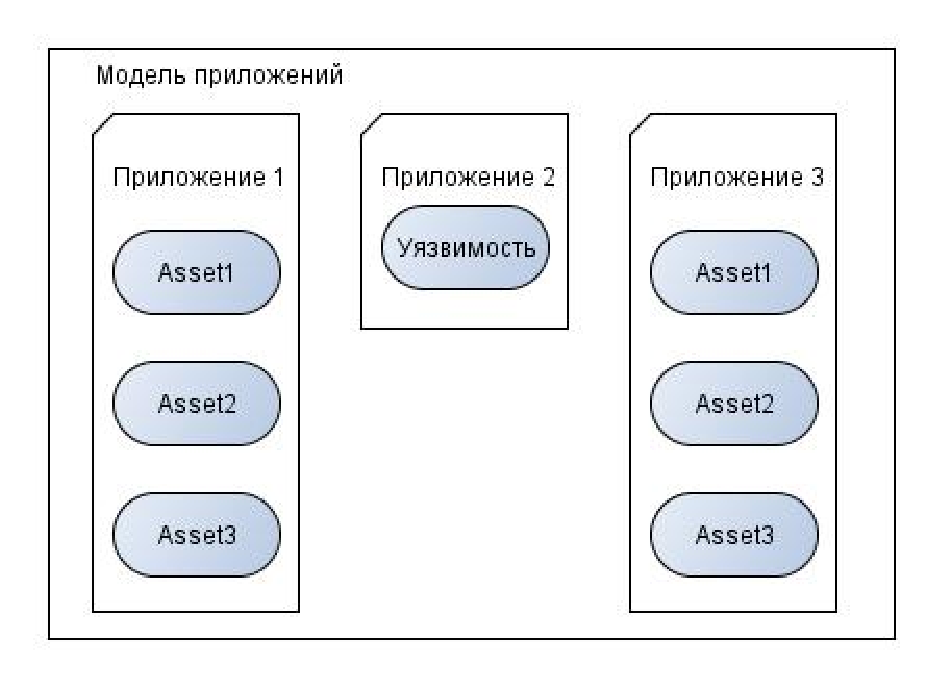
\includegraphics[width = 120mm]{Ch2Pic12}
        \caption{Пятиуровневый стек протоколов.} \label{Pic12}
    \end{figure}

    Модель уязвимости представляет собой вероятностный эксперимент, исход которого зависит от нескольких параметров. Эти параметры разделены на две подгруппы. Первая подгруппа - это характеристики злоумышленника, такие как уровень подготовки, мотив(пен-тест, промышленный шпионаж и.т.д.). Во вторую подгруппу входят параметры, являющиеся информационными. Каждый такой параметр представляет собой информацию, собранную злоумышленником о системе. Данные параметры могут быть как необходимыми для проникновения, так и не влияющими на исход эксперимента. Информация о системе представляется в виде объектов(активов). Эти объекты могут быть получены как путем взаимодействия злоумышленника с целевым сервисом, так и с другими сервисами на рабочей станции, не содержащими уязвимость. Такие сервисы относятся ко второму виду объектов-приложений.

    Второй вид объектов-приложений представлен как модель сервисов, не содержащих уязвимость, но предоставляющих некоторую информацию о системе, которая может быть использована при атаке. Модель такого объекта, как модель объекта, содержащего уязвимость, представляет собой вероятностный эксперимент. Исход этого эксперимента так же зависит от характеристики атакующего.

    В общем виде модель атак, используемая в разрабатываемой системе представляет собой дерево атак(рисунок \ref{Pic13}). Узел $G_{0}$ представляет целевую уязвимость, на которую может быть направлена атака. Каждый узел дерева атаки представляет собой набор промежуточных целей, которые должны быть достигнуты для успешной атаки на главную цель. Промежуточные цели модеут быть представлены в виде И-декомпозиции или ИЛИ-декомпозиции. Цель, представленная ИЛИ-декомпозицией, представляет выбор, при котором должна быть достигнута хотя бы одна из промежуточных целей, для успешной атаки на текущую. Для успеха при атаке на цель, представленную И-декомпозицией, необходимо достижение всех промежуточных целей, которые находятся ниже уровнем.

    \begin{figure}\center
        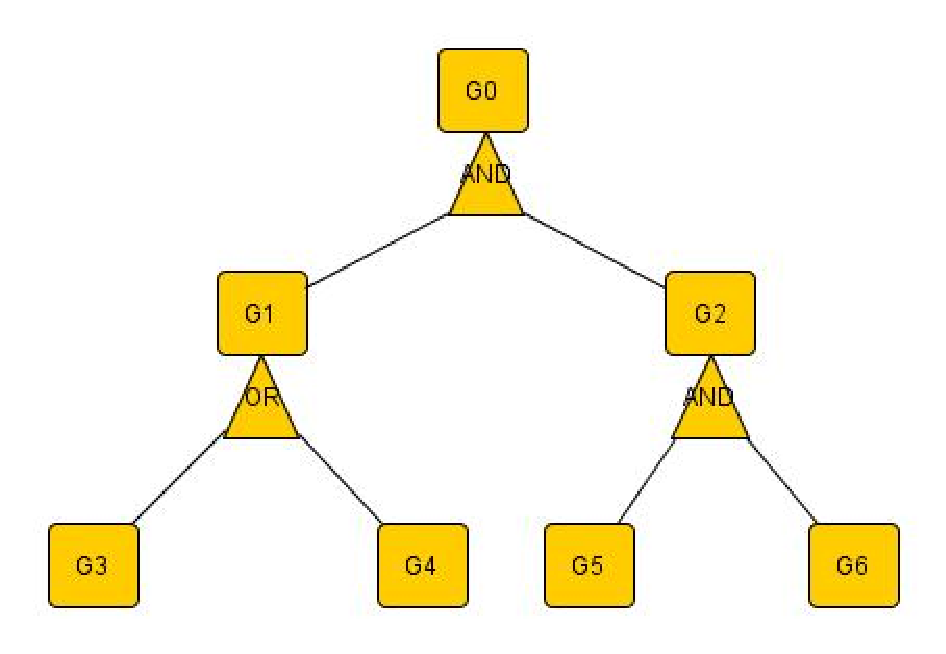
\includegraphics[width = 120mm]{Ch2Pic13}
        \caption{Пятиуровневый стек протоколов.} \label{Pic13}
    \end{figure}

    Рассматривая пример применительно к используемой модели приложений, следует заметить, что узел $G_{0}$ -- это представление первого вида объектов приложений, т.е. объектов, содержащих уязвимость, а $G_{1}$ ... $G_{6}$ -- это приложения, принадлежащие ко второму виду.

    \subsubsection{Модель поведения злоумышленника. }

    Для проведения атаки на компоненты сети передачи данных, злоумышленник должен обладать оборудованием, которое позволит ему совершить провести атаку. Оборудование представляет собой одно или несколько сетевых устройств, чаще всего - рабочих станций, которые имеют доступ в локальную сеть. Оно может быть описано в рамках тех же моделей, которые используются для описания компонентов сети. Главным отличием модели злоумышленника от моделей рабочих станций являются модели приложений. Модель приложений для описания действий злоумышленника включает в себя алгоритм, по которому будет развиваться атака.

    \subsection{Итог. }

    На рисунке ... представлена используемая модель компонентов сети передачи данных, с учетом выделения различных компонент и способа их взаимодействия. Данная модель будет использована при имитации процессов, происходящих в сети передачи данных, в проектируемой системе.

    Система моделирования должна отвечать следующим требованиям:

%    \begin{itemize}
%   \end{itemize}

    Для реализации системы моделирования необходимо:

    \begin{itemize}
        \item Разработать способ описания используемых при моделировании компонентов.
        \item Реализовать описанные модели компонентов предметной области.
        \item Реализовать систему управления, для создания и контроля параметров модели.
        \item Реализовать систему мониторинга за состоянием объектов. Она включает в себя:
            \begin{itemize}
                \item Сбор информации о состоянии очередей приема и отправки данных на объекте.(Возможно с детализацией по уровням)
                \item Сохранение результатов экспериментов.
                \item Отображение результатов атак на приложения.
            \end{itemize}
    \end{itemize}

    %Подробнее!!!

    %Дальнейшие рассуждения касательно модели атак - BRIMSMAADNET - деревья атак.


        %Построение моделей устройств.
        %Каждое устройство, описанное при анализе предметной области должно быть снабжено моделью.

    %?? Системы управления и мониторинга.
    %?? Если говорить про систему принятия решений, то она должна быть упомянута в подсистеме мониторинга.

\end{document} 